

\documentclass{article}

\usepackage[utf8]{inputenc}

\usepackage{amsmath, bm}
\usepackage{graphicx}
\usepackage{amssymb}
\usepackage{float}
\usepackage{caption}
\usepackage{subcaption}
\usepackage{hyperref}
\usepackage{tikz}
\usepackage{layout}

\usepackage[margin=1in]{geometry}
\usepackage{listings}
\usepackage{xcolor}
\usepackage{color, colortbl}
\usepackage{textgreek}
\usepackage{mathrsfs}
\usepackage{booktabs}

\usepackage{titlesec}

\titleformat{\subsubsection}
  {\normalfont\selectfont}{\thesubsubsection}{1em}{}

\usetikzlibrary{calc}
\usetikzlibrary{angles,quotes} % for pic
\usetikzlibrary{patterns,snakes}
\usetikzlibrary{arrows}
\tikzset{>=latex} % for LaTeX arrow head

\setlength{\parskip}{\baselineskip}%
\setlength{\parindent}{0pt}%
\linespread{0.9}


\definecolor{codegreen}{rgb}{0,0.6,0}
\definecolor{codegray}{rgb}{0.5,0.5,0.5}
\definecolor{codepurple}{rgb}{0.58,0,0.82}
\definecolor{backcolour}{rgb}{0.95,0.95,0.92}

\lstdefinestyle{mystyle}{
    backgroundcolor=\color{backcolour},   
    commentstyle=\color{codegreen},
    keywordstyle=\color{magenta},
    numberstyle=\tiny\color{codegray},
    stringstyle=\color{codepurple},
    basicstyle=\ttfamily\footnotesize,
    breakatwhitespace=false,         
    breaklines=true,                 
    captionpos=b,                    
    keepspaces=true,                 
    numbers=left,                    
    numbersep=5pt,                  
    showspaces=false,                
    showstringspaces=false,
    showtabs=false,                  
    tabsize=2
}

\lstset{style=mystyle}



\begin{document}

\title{4A4 Exercise 2}
\author{5739G}
\date{Feburary 2025}
\maketitle

\section{Introduction}

\iffalse
The equations of motion for surge, heave and pitch, in matrix form seen below.

\begin{equation}
  \frac{d}{dt}\left[\begin{matrix}u\\w\\\theta\\q\end{matrix}\right] = \left[\begin{matrix}\frac{X_{u}}{m} & \frac{X_{w}}{m} & - g & \frac{X_{q}}{m}\\\frac{Z_{u}}{m} & \frac{Z_{w}}{m} & 0 & \frac{U m + Z_{q}}{m}\\0 & 0 & 0 & 1\\\frac{M_{u}}{I_{y}} & \frac{M_{w}}{I_{y}} & 0 & 0\end{matrix}\right]
  \left[\begin{matrix}u\\w\\\theta\\q\end{matrix}\right] + 
  \left[\begin{matrix}0\\0\\0\\\frac{M_{\delta e}}{I_{y}}\end{matrix}\right]
  \left[\begin{matrix}\delta_{e}\end{matrix}\right]
\end{equation}

Which is in the state space form $\dot{\mathbf{x}} = \mathbf{Ax+Bu}
\fi

Real flight data was collected from inertial, pitot-static and avionic sensors onboard the SAAB 340B aircraft.
Intentional pilot control inputs were made to excite the aircrafts natural modes.
These pilot inputs are functionally equivilent to disturbance inputs and will be referred to as such.

\section{Modal analysis}

Regions of interest were chosen with little control input (to get the unforced response) and small deviations from equilibrium to stay within linear theory.
The rate of change of angles were favoured over the angles themselves because they are directly measured from rate gyros rather than reconstructed from kalman filters.
In many cases the derivatives also had higher amplitudes and so gave less absolute uncertainty in measurements.

\begin{figure}[H]
  \centering
  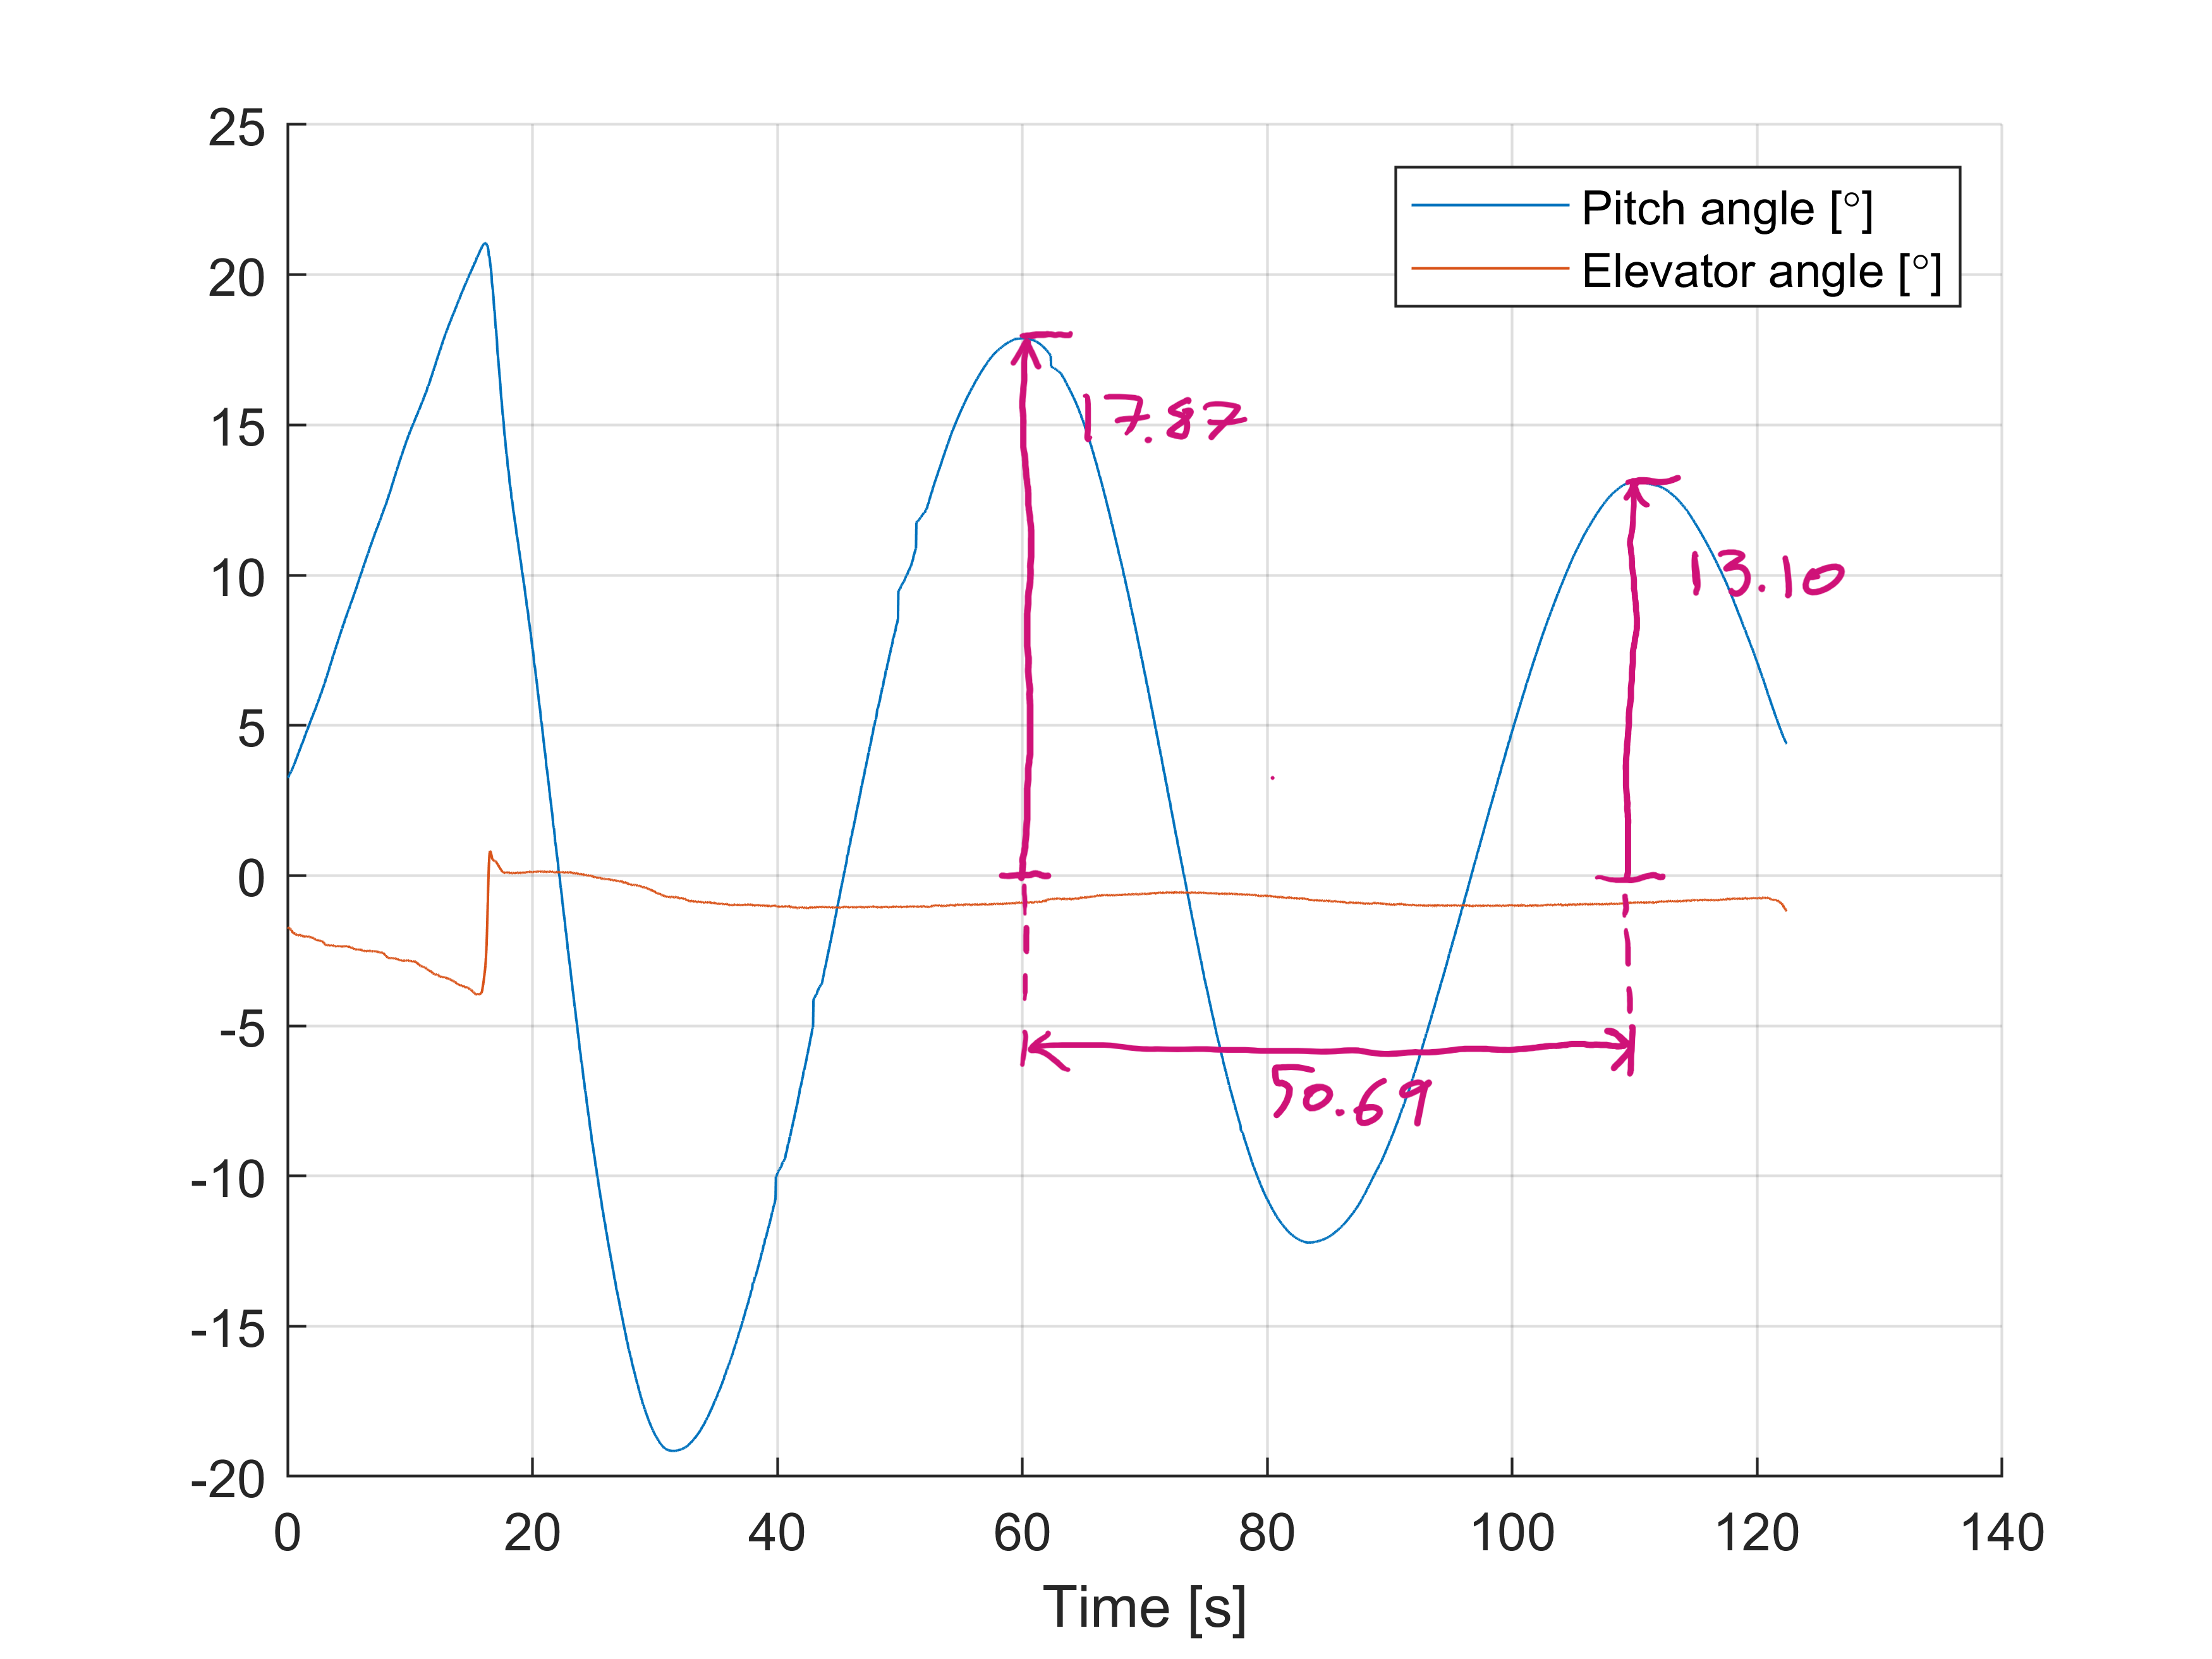
\includegraphics[width=0.8\textwidth]{figures/anPhugoid.png}
  \caption{Aircraft pitch response to disturbance in elevator angle showing the Phugoid mode.}
  \label{fig:phugoid}
\end{figure}

The transient peak ratios calculated from figure \ref{fig:dutchroll} are 0.812, 0.841.
This gives an average of 0.827, which using figure \ref{fig:tpr_to_zeta}, corresponds to a damping ratio of 0.06.
The average period is 51.42 seconds and finally using equation \ref{eq:tpr_freq} gives $\omega_n = 0.126$.
\begin{equation}
  \omega_n = \frac{2 \pi}{T\sqrt{1 - \zeta^2}}
  \label{eq:tpr_freq}
\end{equation}
The control elevator input can be seen to vary slightly over the region considered but is likely small enough to have confidence in the values measured from the graph.
The damping ratio determined using figure \ref{fig:tpr_to_zeta} would have a high uncertainty, however the small value of $\zeta$ means that the natural frequency is not significantly affected.

\begin{figure}[H]
  \centering
  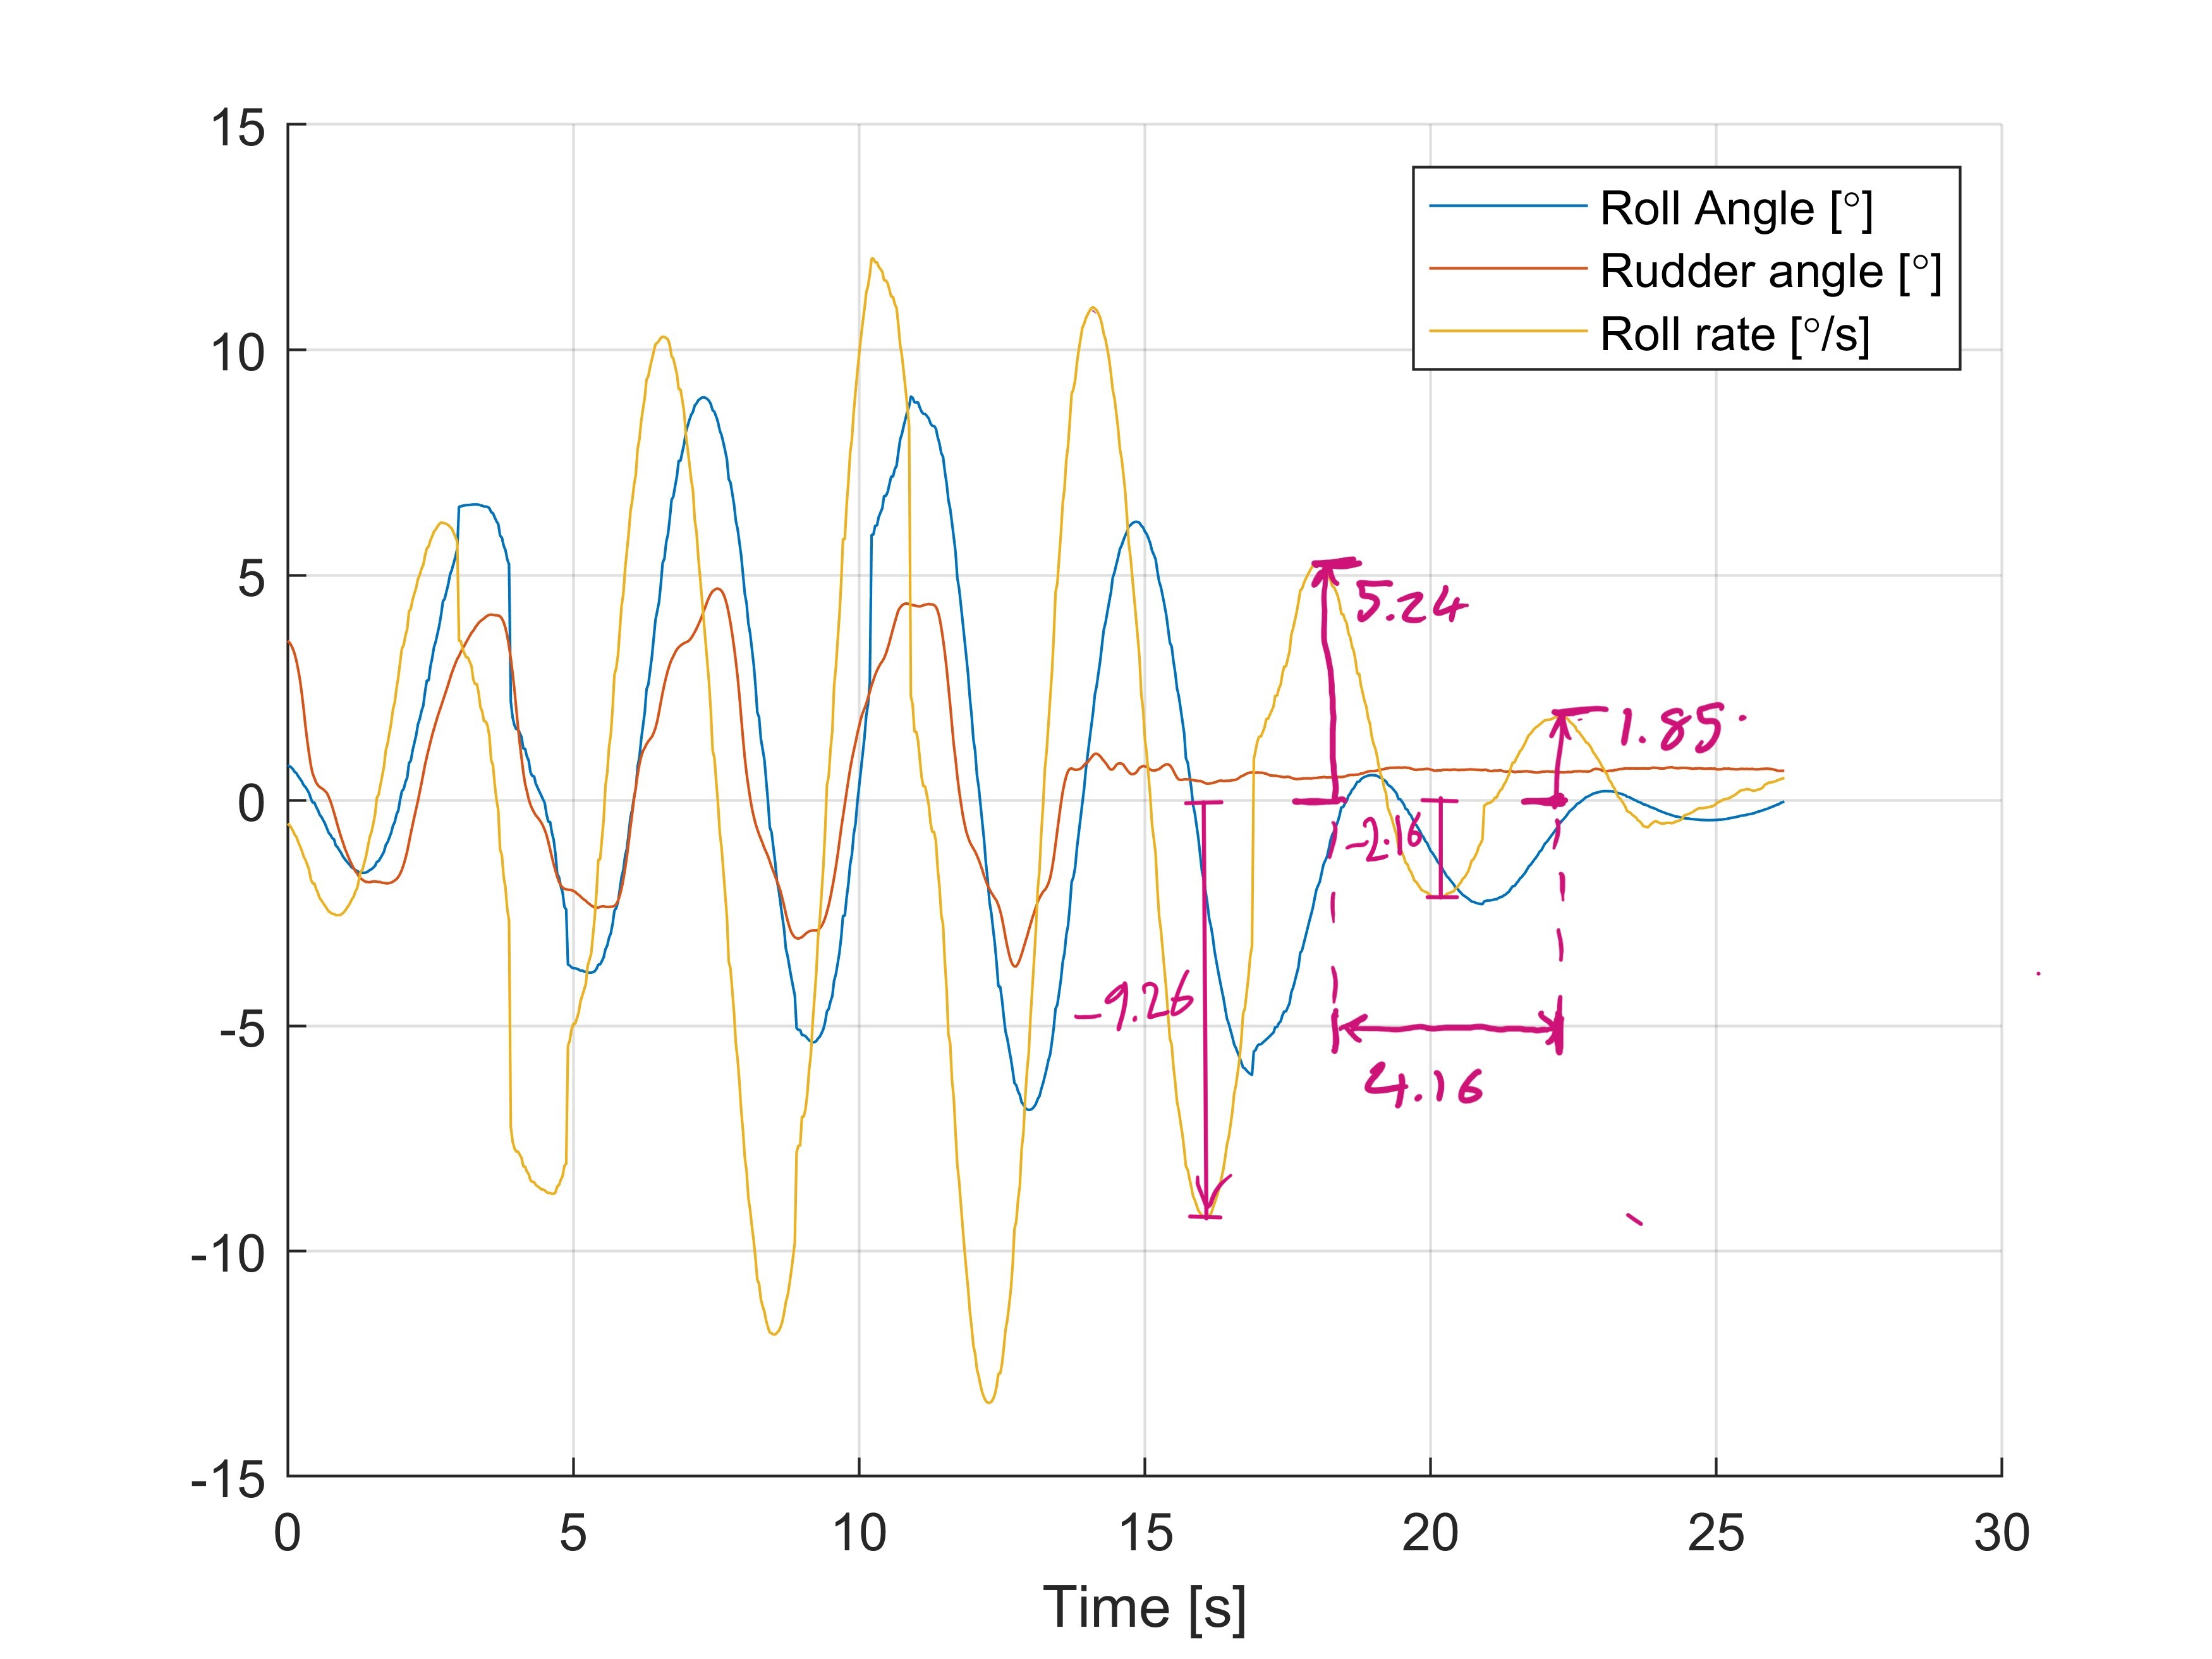
\includegraphics[width=0.8\textwidth]{figures/anDutchRoll.jpg}
  \caption{Aircraft roll response to sinusoidal rudder disturbance showing the Dutch Roll mode.}
  \label{fig:dutchroll}
\end{figure}

The transient peak ratios calculated from figure \ref{fig:dutchroll} are 0.719, 0.648, 0.542.
This gives an average of 0.695, corresponding to a damping ratio of $\zeta = 0.12$.
The natural frequency is then found using the equation \ref{eq:tpr_freq} with $T=4.16$ from figure \ref{fig:dutchroll}
This is then calculated to be $\omega_n = 1.52$ rad/s.

The control rudder input is constant over the region considered and an additional peak means that the peak ratios and time period should be more accurate than the previous phugoid modes.
A larger damping ratio means that the uncertainty from the peak ratio graph is larger but this is still not expected to be significant.

\begin{figure}[H]
  \centering
  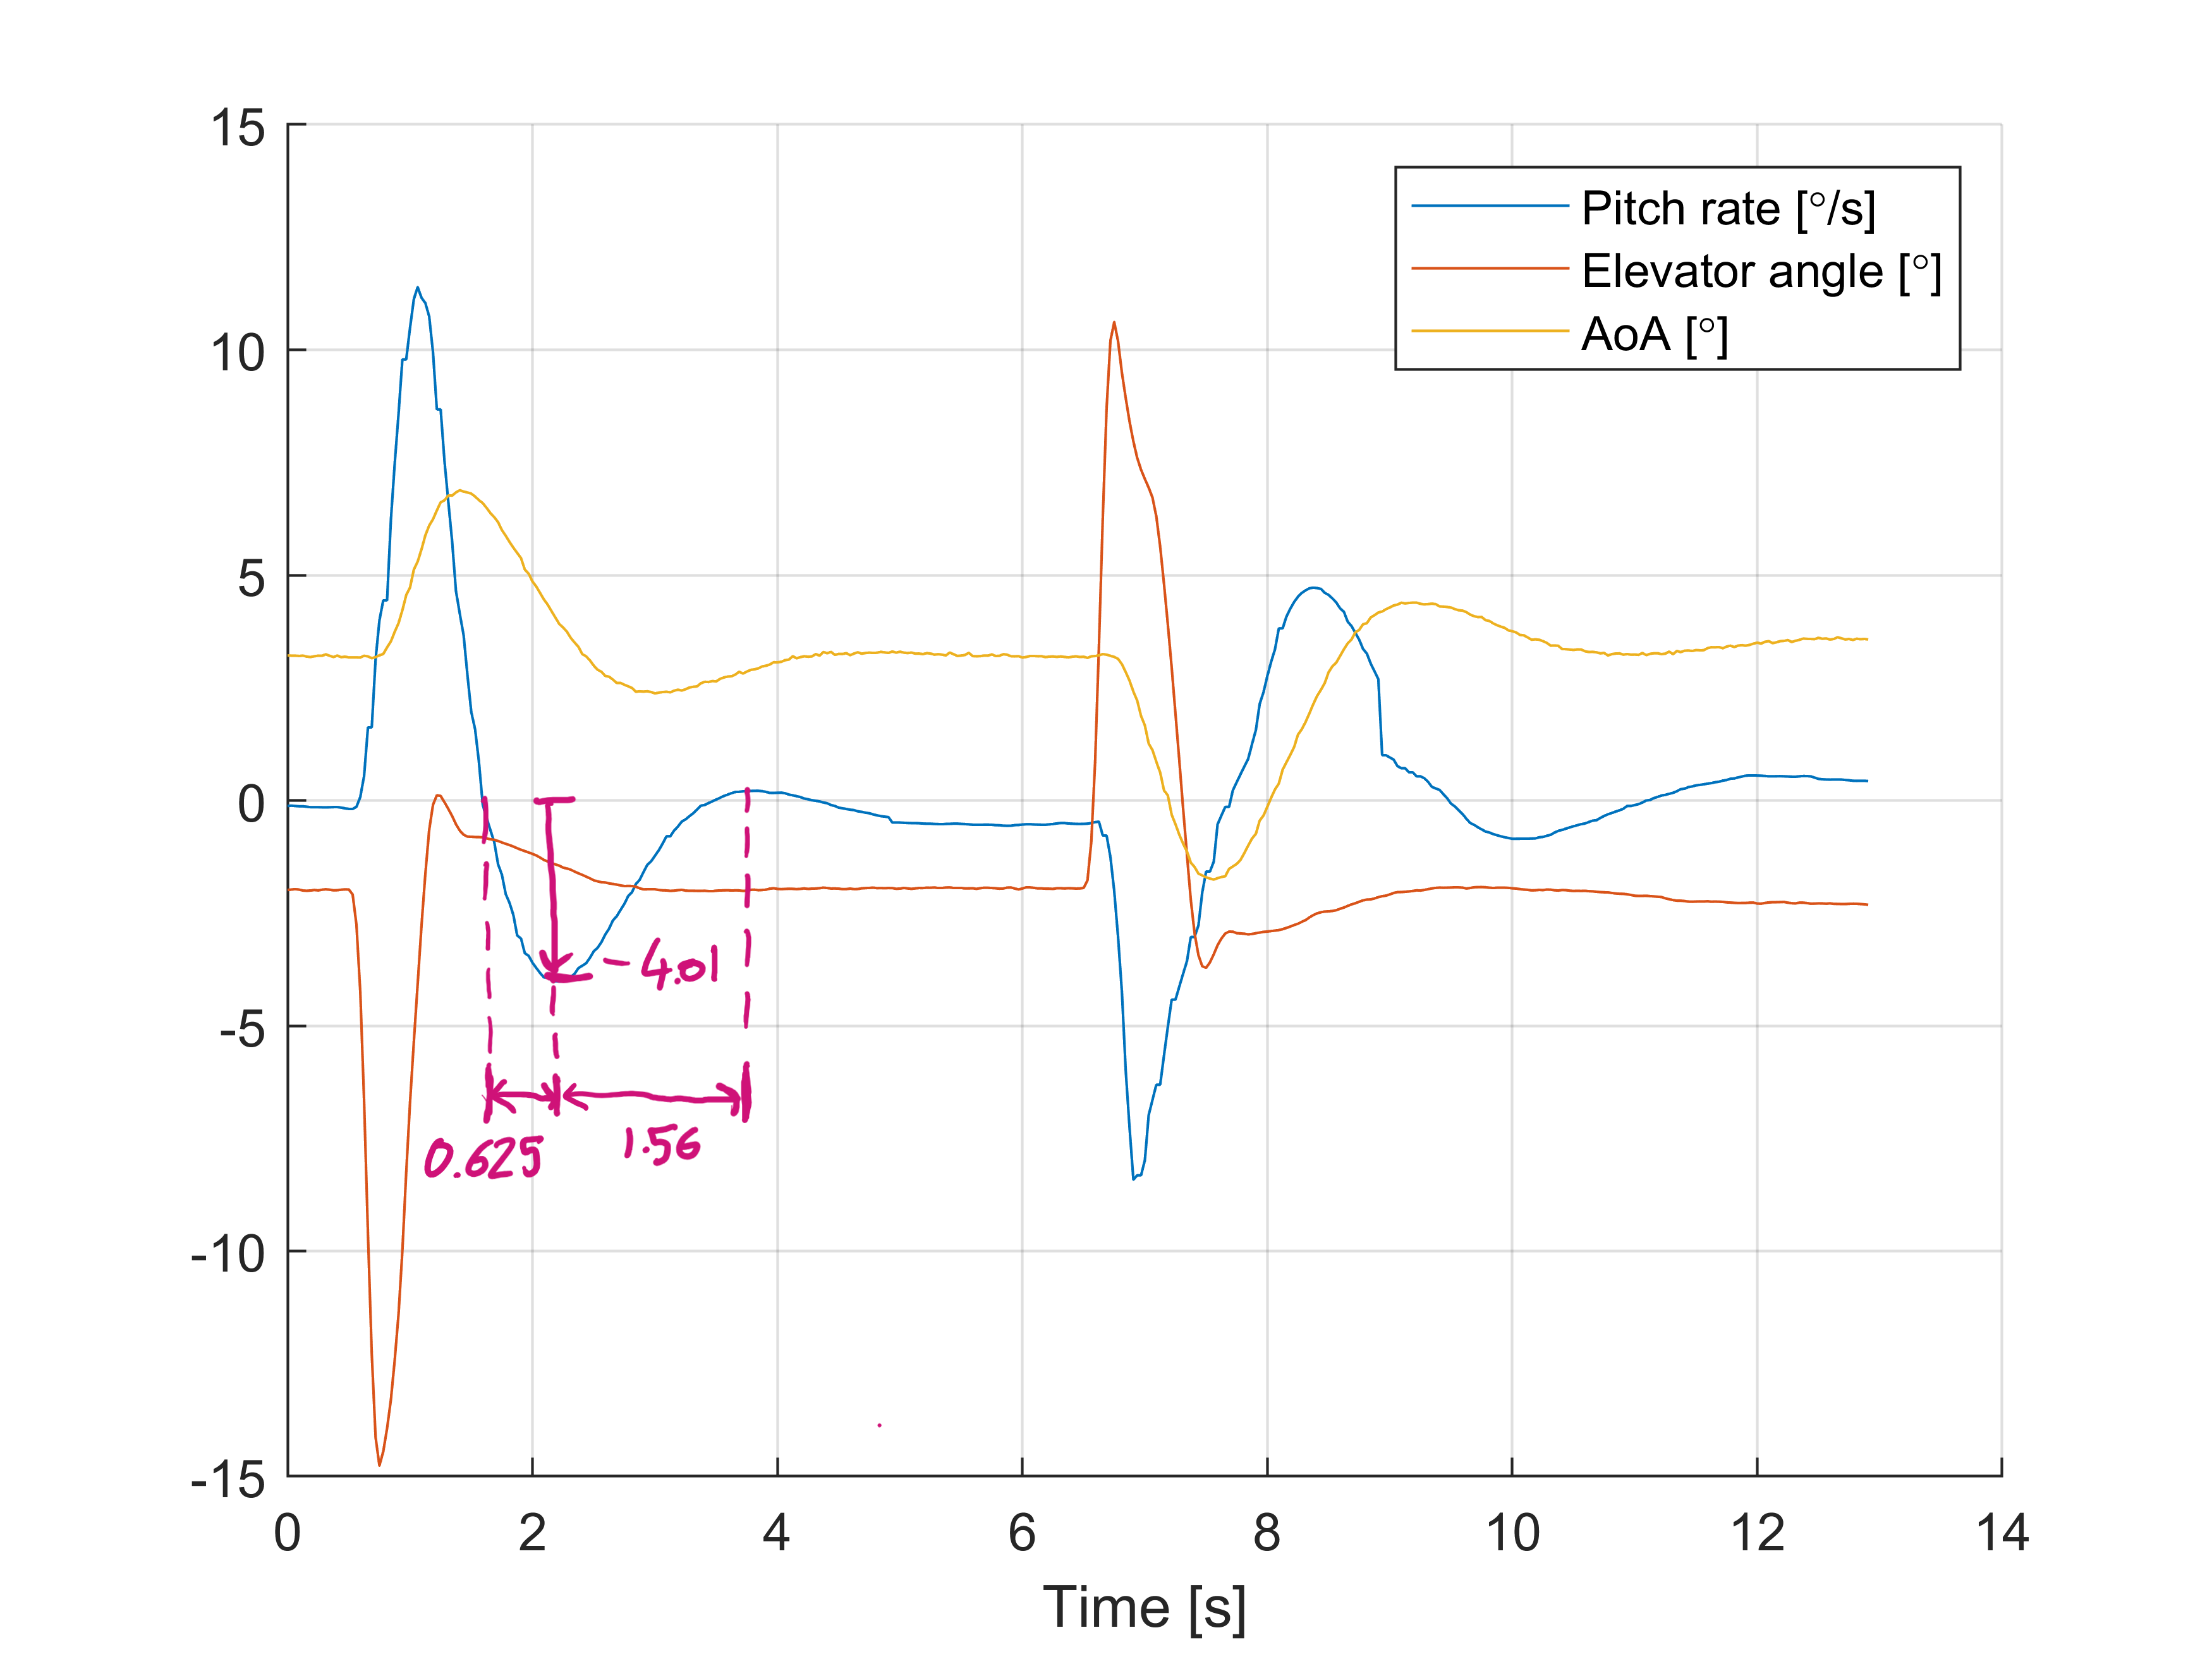
\includegraphics[width=0.8\textwidth]{figures/anSPO.png}
  \caption{Aircraft pitch rate response to impulse elevator disturbance showing Short Period Oscillation (SPO) mode.}
  \label{fig:spo}
\end{figure}

This short period oscillation is highly damped and so is harder to obtain accurate modal characteristics.
The unforced part of the response, shown anotated in figure \ref{fig:spo} is matched to a decaying sine-wave shown in equation \ref{eq:spoeq}.
\begin{equation}
  y = Ae^{-\zeta\omega_{n}(t - t_{0})}\sin(\omega_{d}(t - t_{0})) + B
  \label{eq:spoeq}
\end{equation}
Where
\begin{equation}
  \omega_{d} = \omega_{n}\sqrt{1 - \zeta^{2}}
\end{equation}
From the graph $t_0 = 1.625$, $B=-0.54$ and $\omega_d = \pi/1.56 = 2.014$.
The damping ratio is then a function of the phase of the first peak, $\psi_m = 0.56\omega_d$.
\begin{equation}
  \tan(\psi_m) = \frac{\sqrt{1-\zeta^2}}{\zeta}
\end{equation}
Rearranging and taking positive root gives $\zeta= 0.4286$.
Then using the amplitude $y(t=t_0 + 0.56) = -3.47$ we could solve for $A$ but this isnt required.

Multiple single point graph measurements are used to calculate the SPO which propagates a significant amount of error.
The short period oscillation mode parameters are therefor presented with high uncertainty.

\begin{figure}[H]
  \centering
  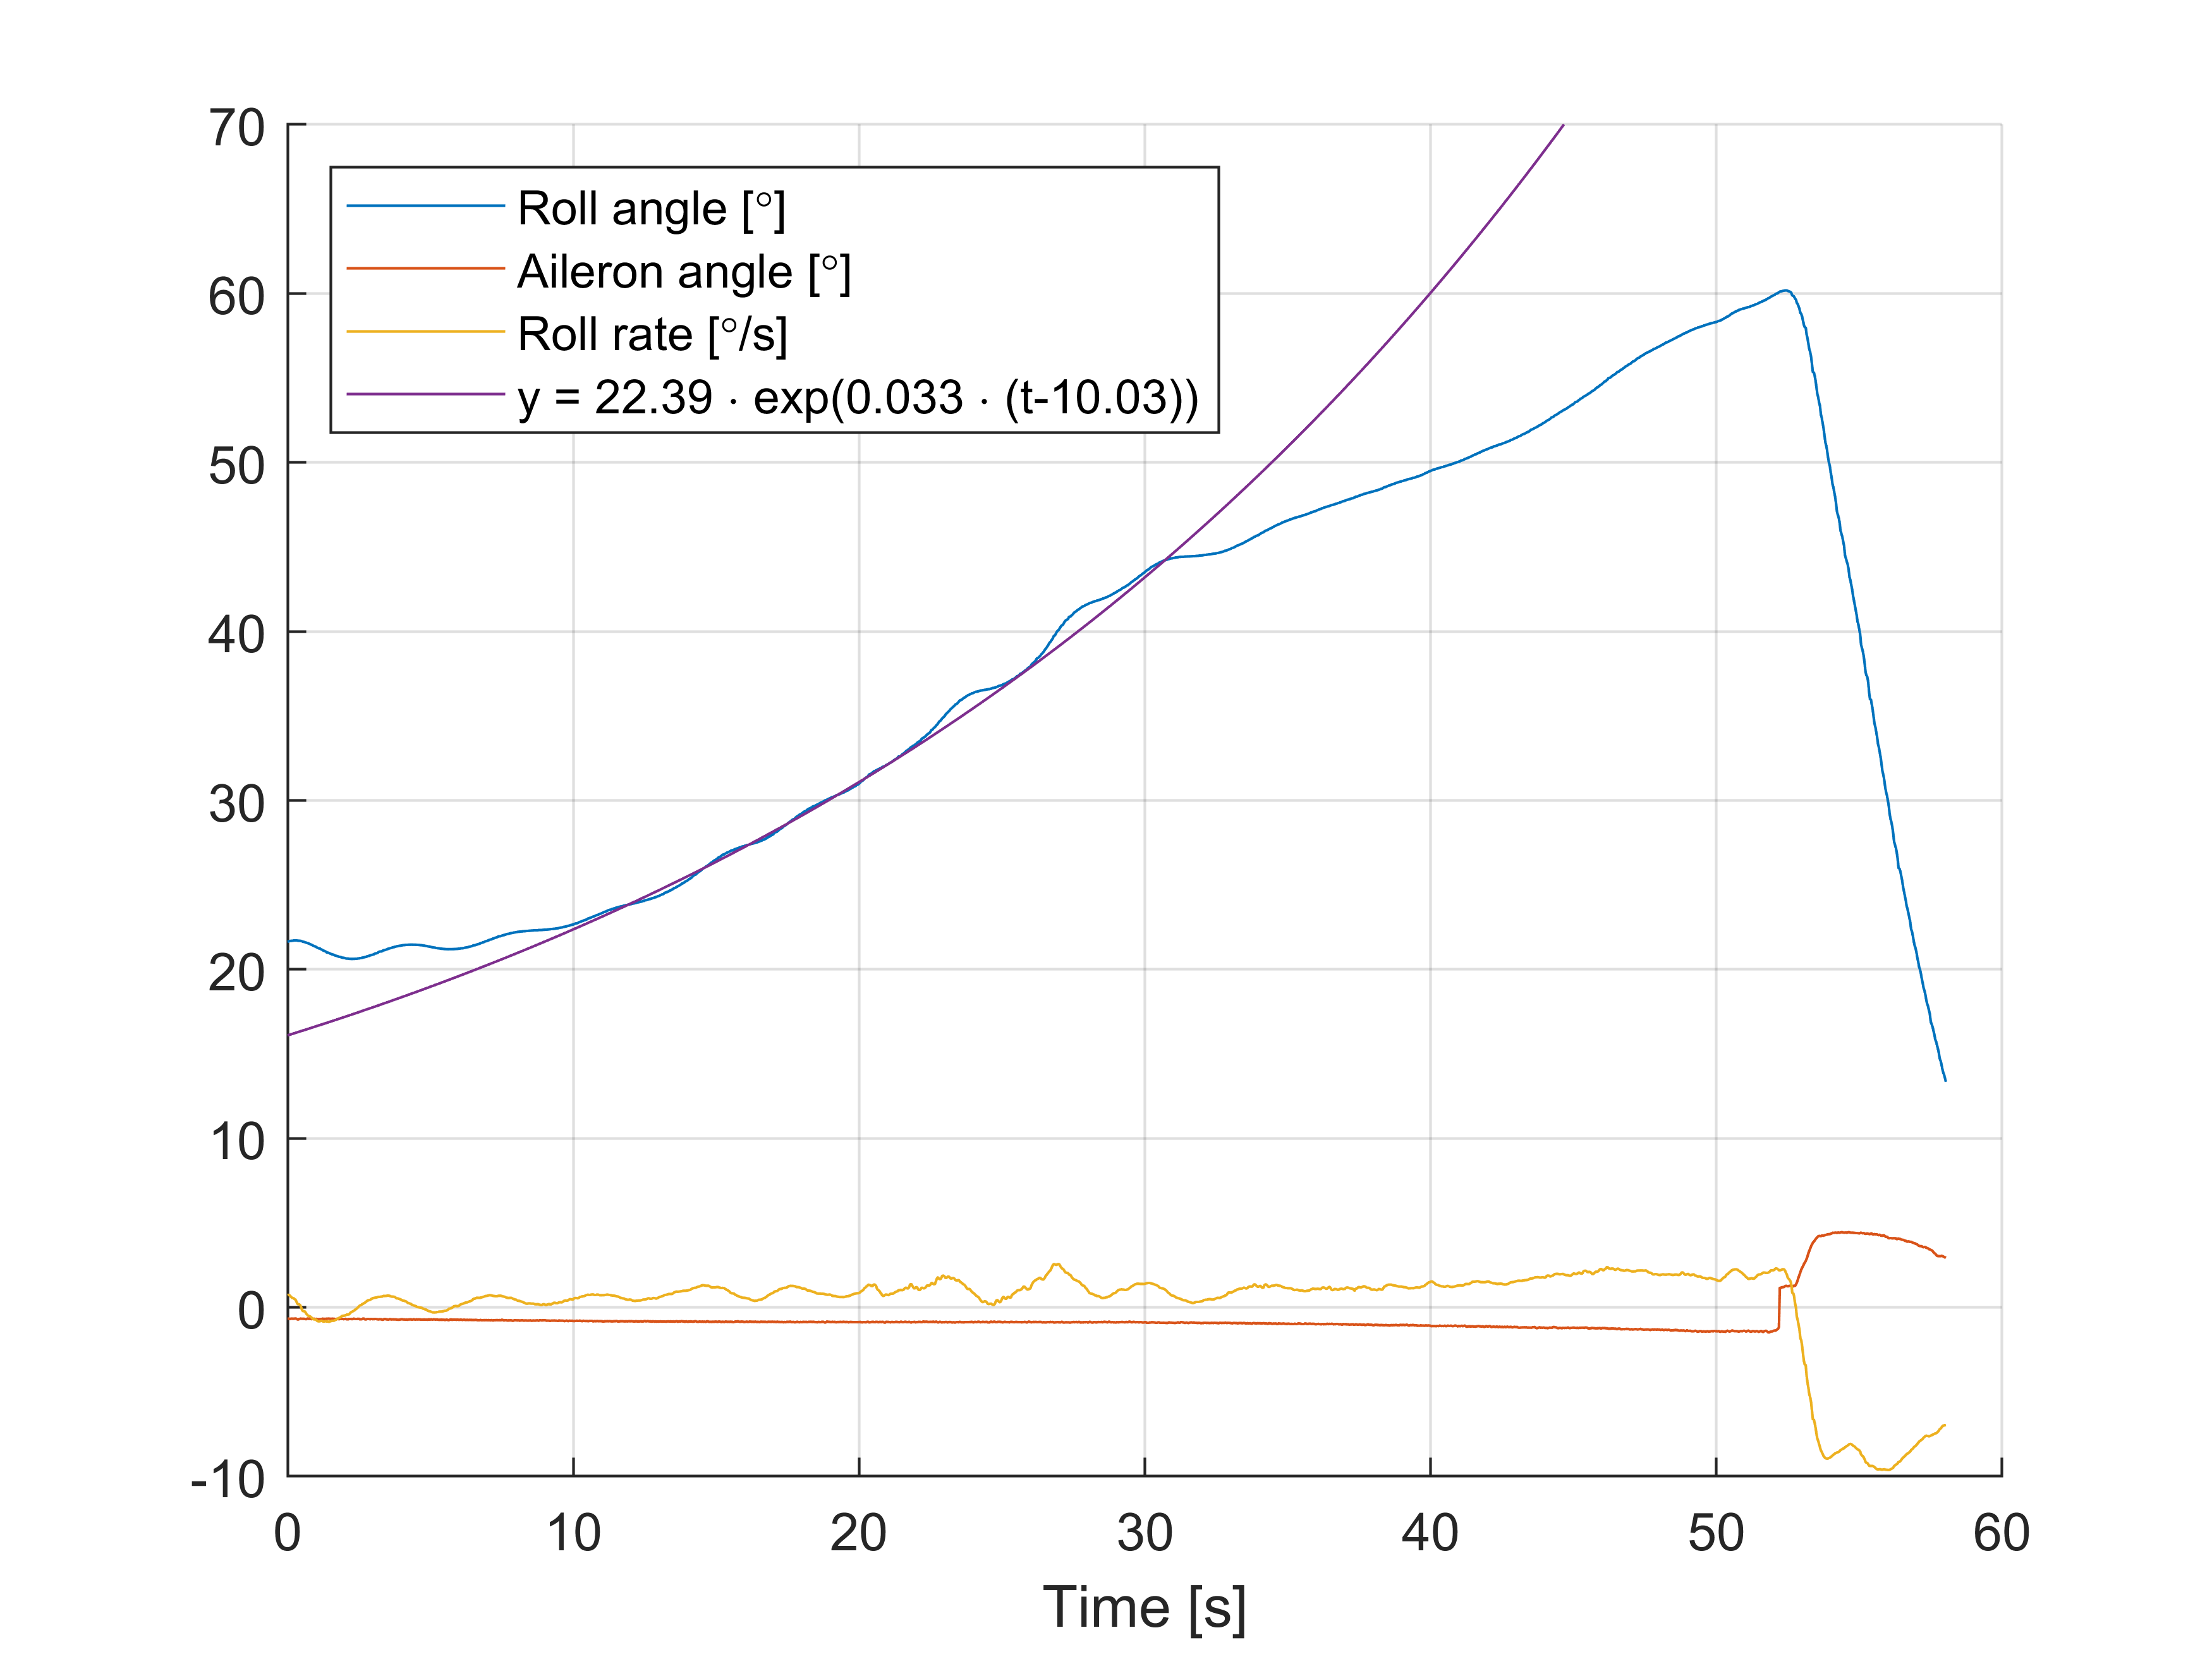
\includegraphics[width=0.8\textwidth]{figures/Spiral.png}
  \caption{Roll angle response at high bank angle showing the Spiral mode.}
  \label{fig:spiral}
\end{figure}

\begin{figure}[H]
  \centering
  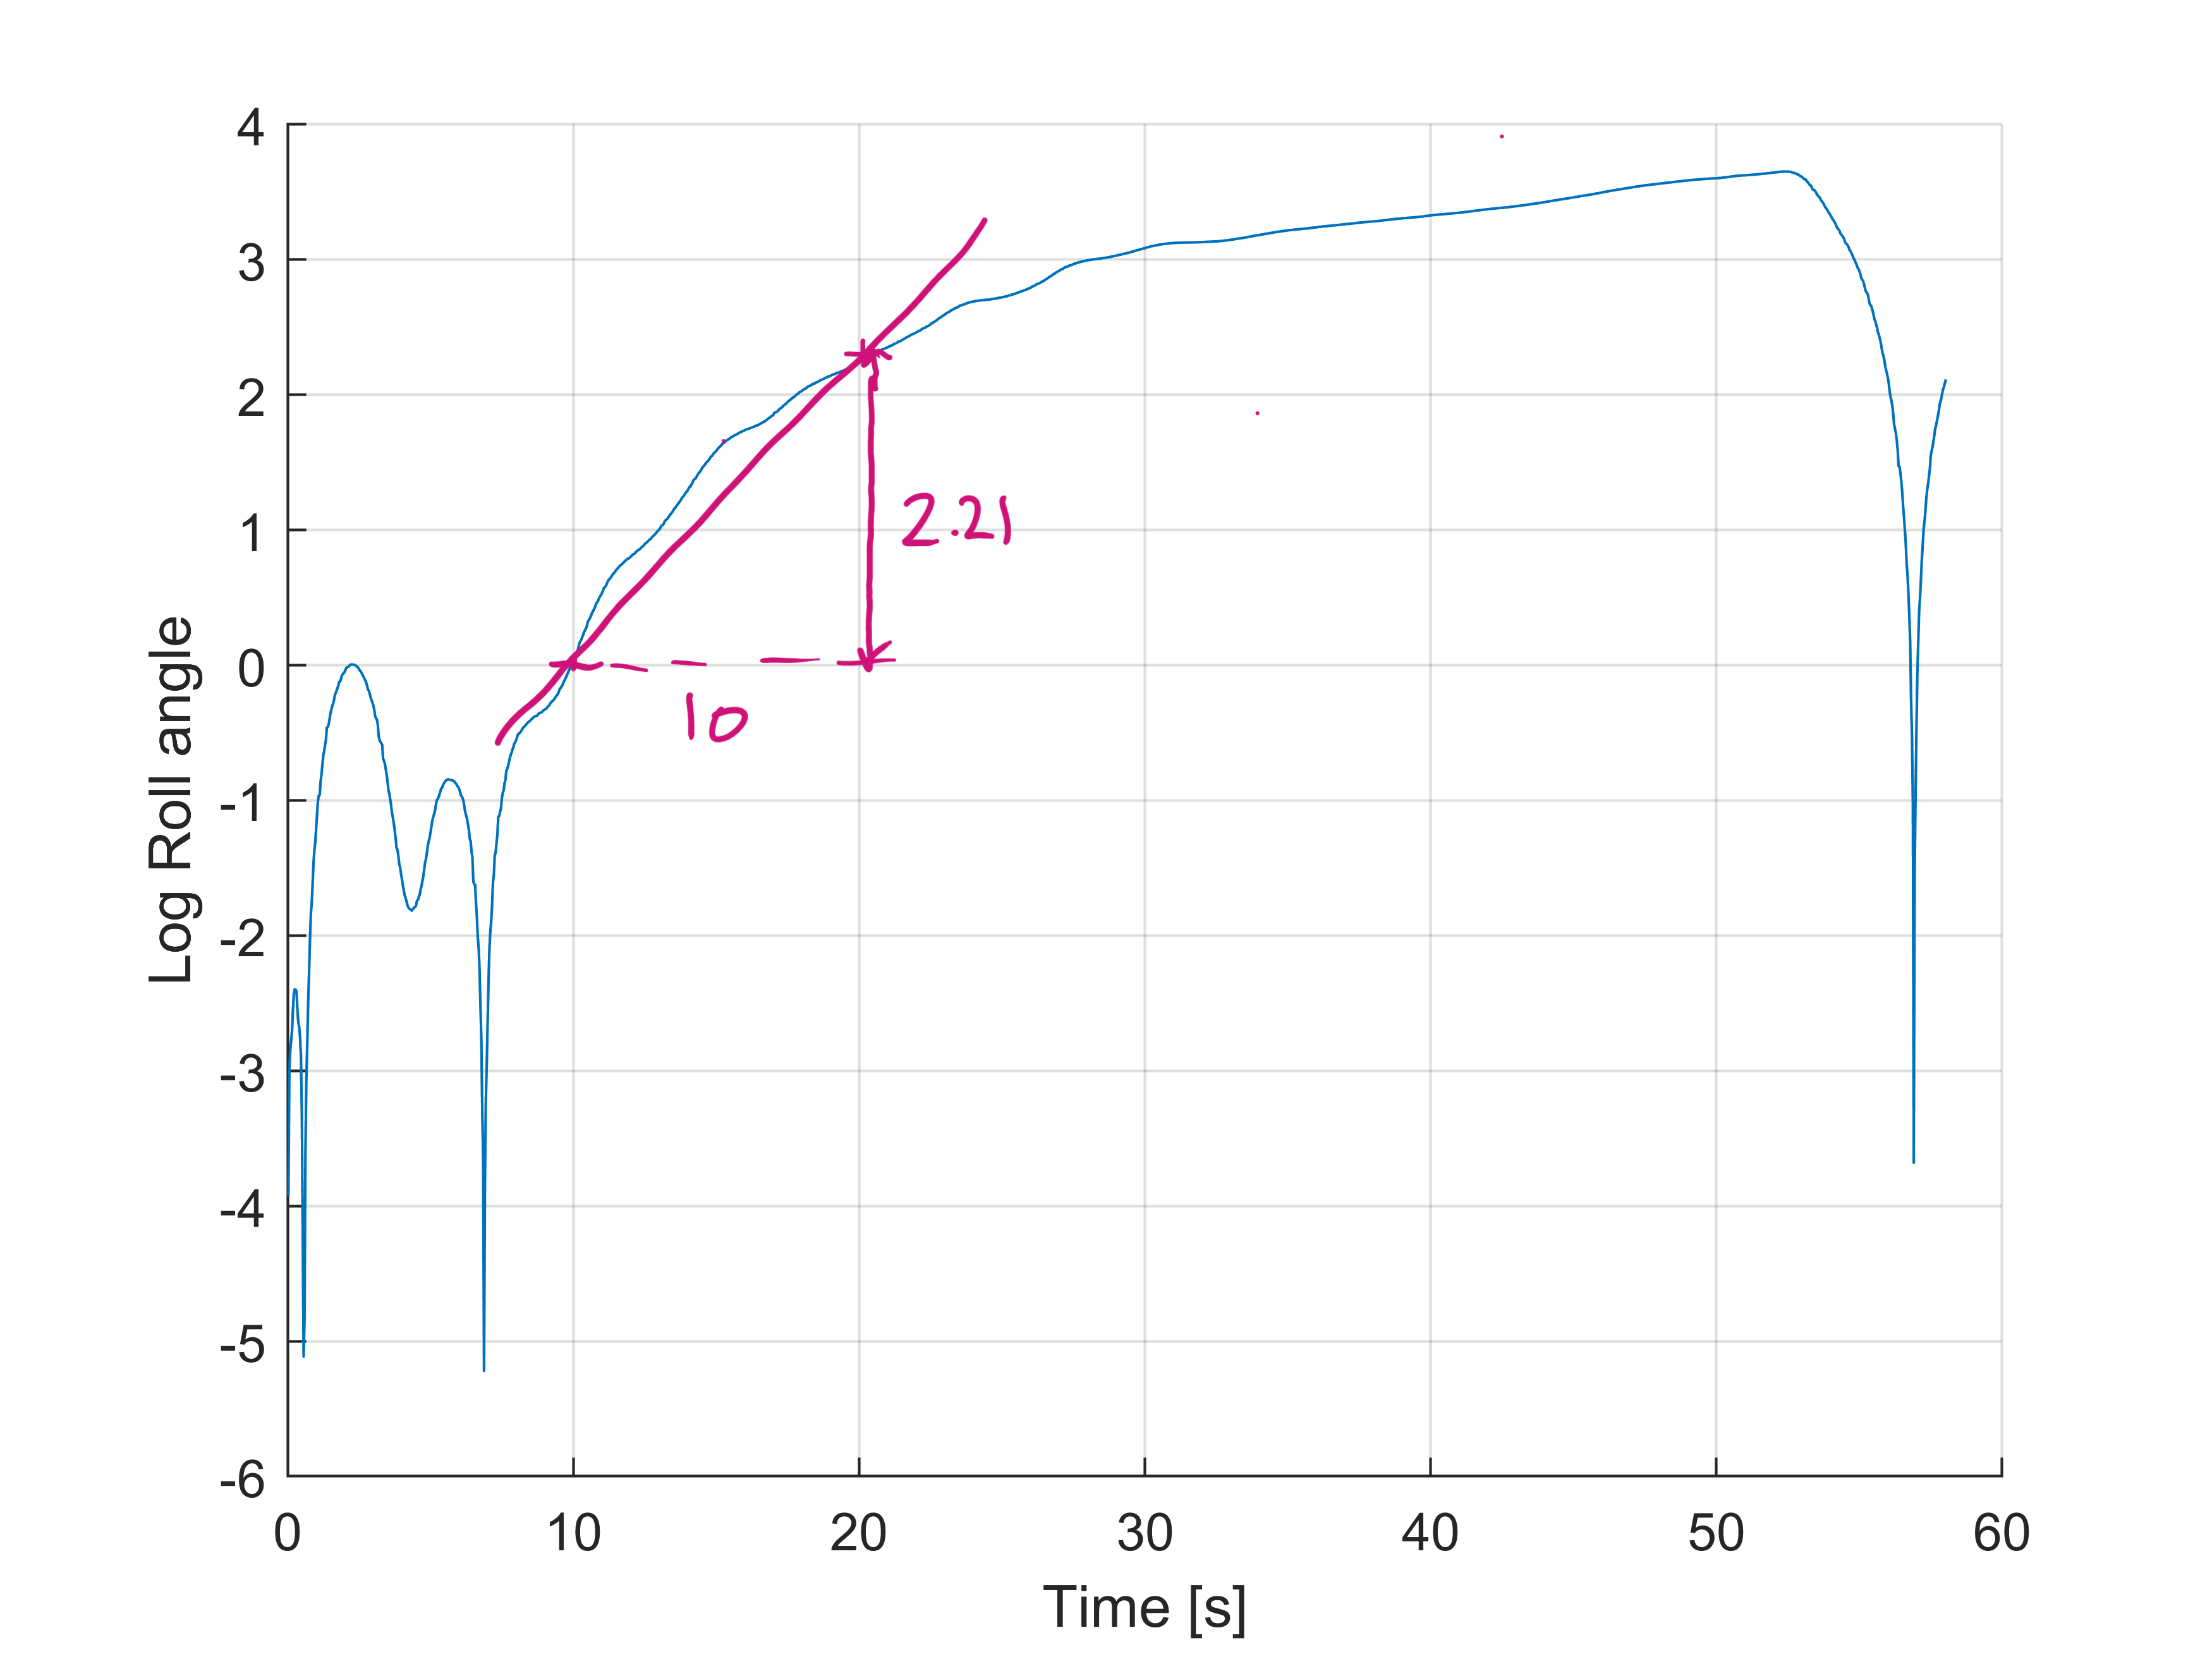
\includegraphics[width=0.8\textwidth]{figures/anSpiral_log.png}
  \caption{$\log(\texttt{Rollang} - \texttt{Rollang}(1))$ against $\texttt{Time}$ for exponential curve fitting.}
  \label{fig:spiral_log}
\end{figure}

Manual curve fitting was attempted by plotting $\log(\texttt{Rollang} - \texttt{Rollang}(1))$ against $\texttt{Time}$ to obtain the time constant.
The gradient was taken at the start to be in the linear region.
This however showed poor agreement with the data and so instead MATLABs curve fitting toolbox was used to fit the data to an exponential curve seen in figure \ref{fig:spiral}.
The fit was done over the region between 10 and 30 seconds to avoid the initial transient.
This gave a time constant of 30.31 seconds.

The root mean square error of the fit is found to be 0.198 and so agrees well with the data.
However, this is for large bank angles and may exhibit non-linear behaviour which is not accounted for in the model.
For this reason its hard to have confidence in the time constant obtained.

\begin{figure}[H]
  \centering
  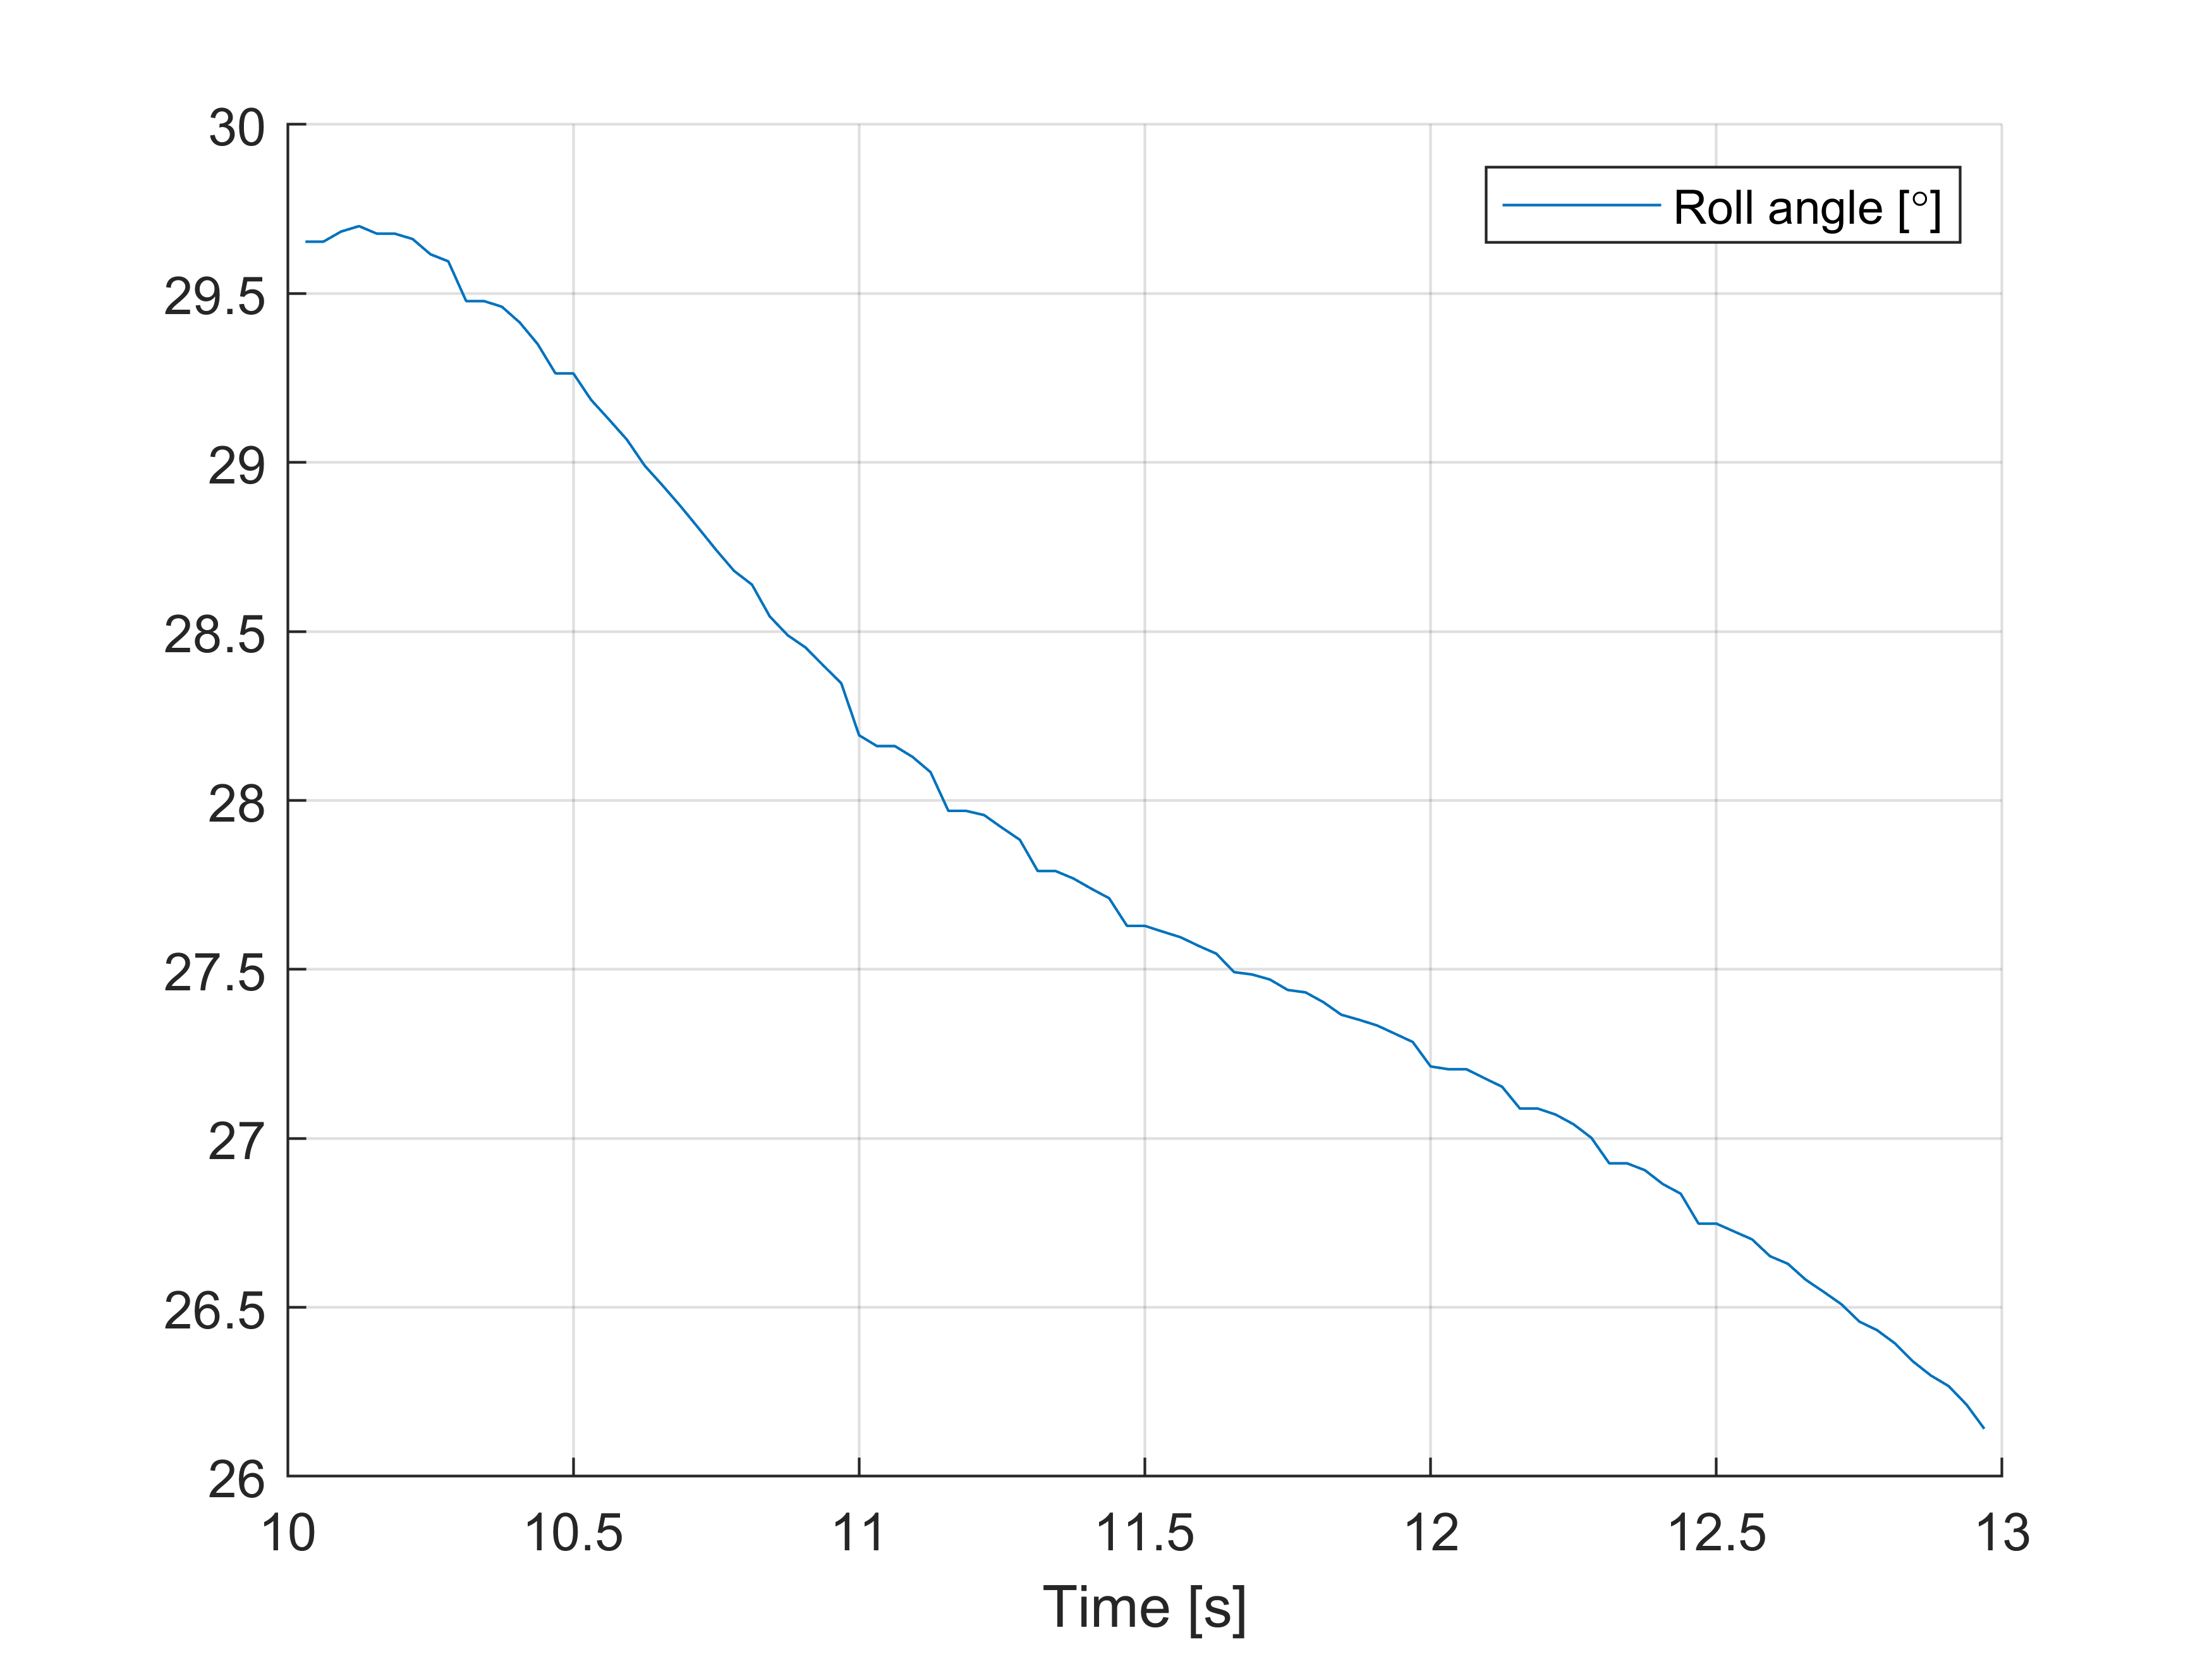
\includegraphics[width=0.8\textwidth]{figures/RollSubs.png}
  \caption{Roll angle response to step elevator disturbance}
  \label{fig:rollsubs}
\end{figure}

The equation fitted in figure \ref{fig:rollsubs} can be rearranged to
\begin{equation}
  y(t) = 22.30 + 3.75(1 - \exp(0.659 (t - 10.22)))
\end{equation}
This corresponds to a time constant of 1.52 seconds.

The root mean square error of the fit is found to be 0.178 and so again the fit agrees well with the data.
The small window size alongside previously mentioned non-linear behaviour at large roll angles means that its difficult to have confidence in the time constant obtained.

\section{Summary of Results}

\begin{table}[H]
  \centering
  \begin{tabular}{lcc}
      \toprule
      Name & Damping factor & Natural frequency (rad/s) \\
      \midrule
      Phugoid & 0.06 & 0.126 \\
      Dutch Roll & 0.12 & 1.52 \\
      SPO & 0.429 & 2.23 \\
      \bottomrule
  \end{tabular}
  \caption{Oscillatory Modes}
\end{table}

\begin{table}[H]
  \centering
  \begin{tabular}{lc}
      \toprule
      Name & Time constant (s) \\
      \midrule
      Spiral & 30.31 \\
      Roll Subsidence & 1.52 \\
      \bottomrule
  \end{tabular}
  \caption{Non-Oscillatory Modes}
\end{table}

\section{Conclusion}

Modal analysis on real data from the SAAB 340B aircraft has been performed.
The methods used to obtain and resultant parameters are presented.
Comments on the accuracy of parameters are also given.

\section{Appendix}

\begin{figure}[H]
  \centering
  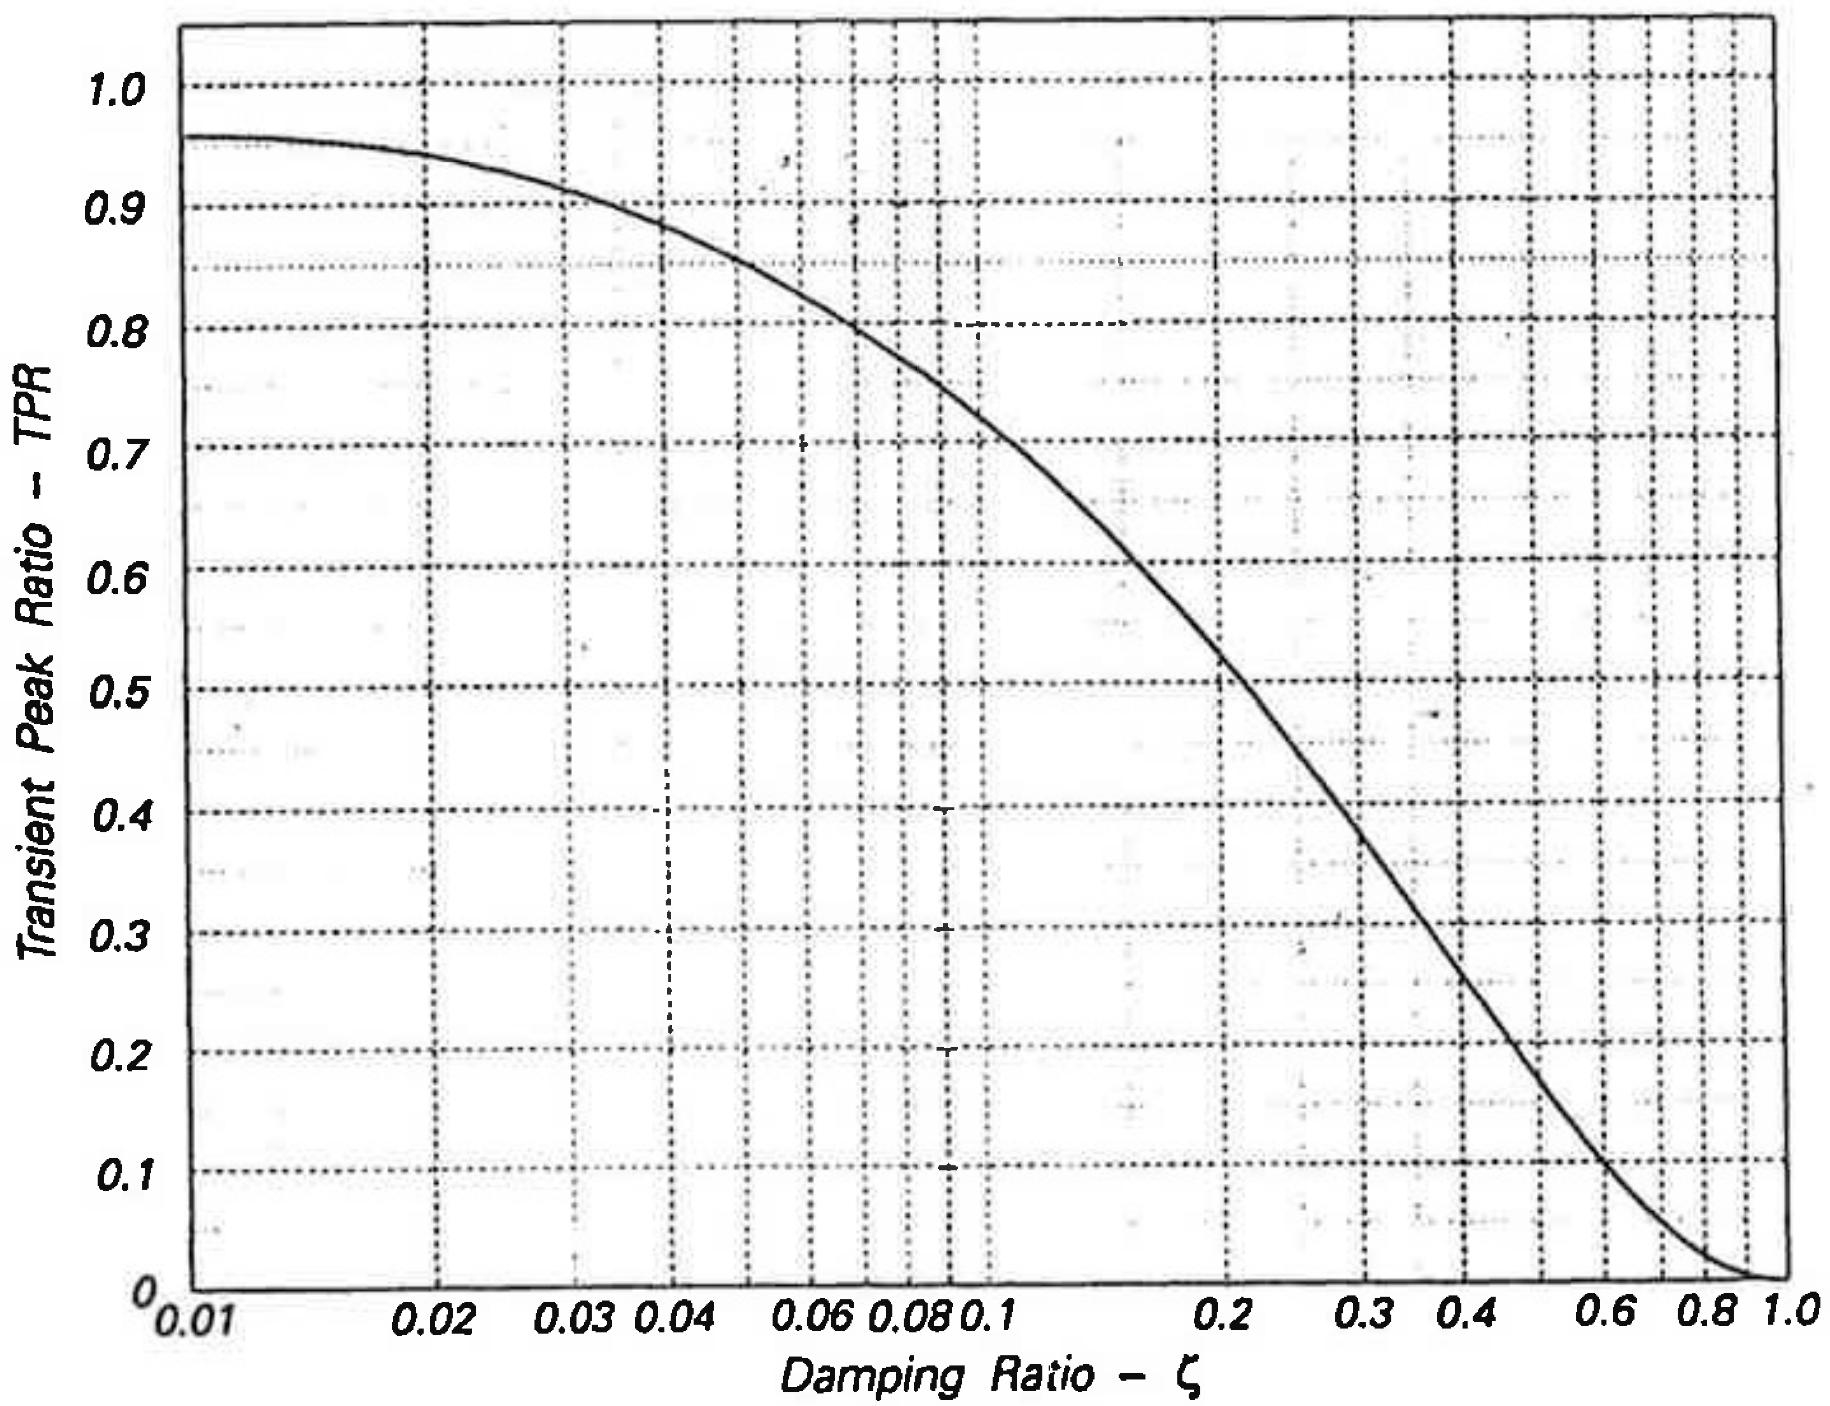
\includegraphics[width=0.6\textwidth]{figures/tpr_zeta.png}
  \caption{Damping ratio from transient peak ratio (TPR) \cite{?}}
  \label{fig:tpr_to_zeta}
\end{figure}

\begin{thebibliography}{9}

  \bibitem{handout}
  S. Place, A. Cooke
  \emph{Flight Experimental Methods: Course Handbook}
  Cranfield University,

\end{thebibliography}

\end{document}

